\section{Experimental Evaluation}

In this section, we will empirically evaluate the performance of known approximation algorithms for item pricing and bundle pricing. Our goal is to understand the behavior of the algorithms on practical \texttt{SQL} queries over real world datasets as well as the behavior on random hypergaphs. We will first describe our experimental setup, followed by the various knobs that we can control to create different instances of the hypergraph instances and valuations. 

\subsection{Experimental setup}

We perform all our experiments on $2.2$ GHz processor machine with $4$ cores and $16$ GB main memory running OS X $10.10.5$. \texttt{MySQL} is used as the underlying database for query processing and evaluation . Our implementation is written in \textsc{Python} as an enhancement in \textsc{Qirana} prototype system. \textsc{Qirana} generates random neighbors of a database as its support set over which query pricing is performed. The advantage of using neighbors is that we can succinctly represent the neighbor without storing the new database, i.e, we can represent the neighbor by storing only the \emph{update query} that generates the neighboring database. Thus, given a query $\bQ$ and support set $\mS$ for database $\db$, \textsc{Qirana} will compute the conflict set of the query. Then, the system will assign prices to each item in the conflict set.
Table~\ref{table:experiments} shows the experimental design space we consider. Our experiments will be over three different datasets. For each dataset and valuation model (which in turn will use different distributions), we compute the revenue that can be extracted using the algorithms listed. In order to compare different algorithms we use two upper bounds: $(i)$ sum of valuations, and $(ii)$ an upper bound on the optimal subadditive valuation. We find an upper bound on the optimal subadditive valuations by computing a linear program whose constraints encode the arbitrage constraints. Since the number of constraints can be exponential in the number of hyperedges, we optimize by greedily adding constraints for bundles with largest valuations and finding a set of bundles that cover the hyperedge with small valuations. As we will see later, this helps us compare the performance of algorithms with respect to the subadditive bound that can be better than sum of valuations. In all our experiments, we report each data point as an average over $5$ runs where we discard the first run to minimize cache latency effects.

\begin{table*} \centering
	\def\arraystretch{1.35}%
	\begin{tabular}{c|c|c|c}
		\toprule
		\textbf{Dataset} & \textbf{Algorithms} & \textbf{Workload} & \textbf{Valuation Model}\\ \midrule
		$\texttt{\bfseries world}$ dataset & Uniform Bundle Pricing & SQL query workload & Sampled Bundle Valuations \\ 
		& Uniform Item Pricing & Random workload & Scaled Bundle Valuations \\ 
		& Item Pricing LP &  & Additive Bundle Valuations \\ 
		& Limited Supply LP & &  \\
		& Layering &  &  \\
		\bottomrule
	\end{tabular}
	\caption{Experimental Design Space}
	\label{table:experiments}
\end{table*}

\subsection{Workload and Dataset Characteristics}

\begin{figure}[!h]
	
	\begin{minipage}[t]{0.49\linewidth}
		\centering
		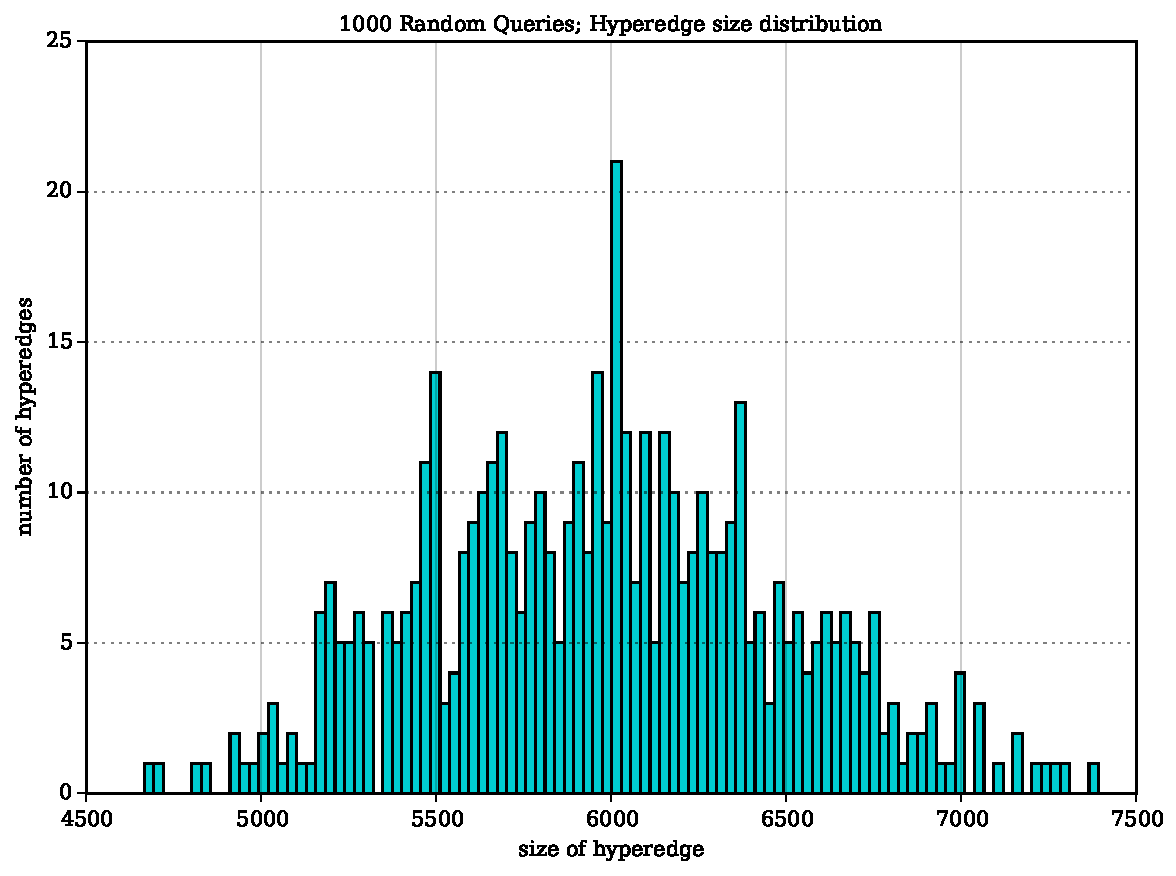
\includegraphics[scale=0.35]{histogramhyperedgesizerandomworkload.pdf}
		\caption{Random workload} \label{fig:histogramrandom}
	\end{minipage}
	\begin{minipage}[t]{0.47\linewidth} 
		\centering
		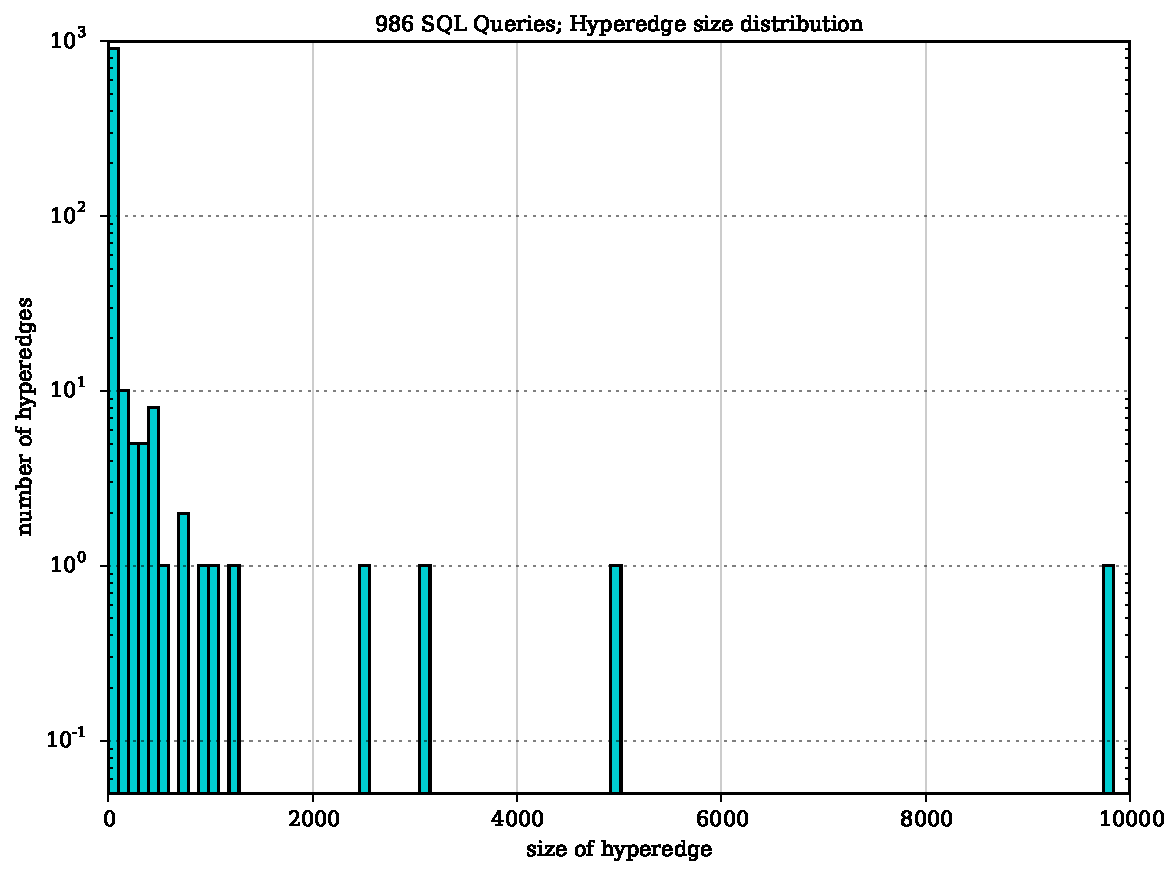
\includegraphics[scale=0.35]{histogramsqlworkload.pdf}
		\caption{SQL workload} \label{fig:histogramrealqueries}
	\end{minipage}        
\end{figure}  

\begin{table*}[] \centering
	%\ra{1.3}
	\begin{small}
		\begin{tabular}{@{}lrrr@{}}\toprule
			\textbf{Workload} & \textbf{\# Queries} & \textbf{Maximum Item Degree} & \textbf{Average edge size} \\ \midrule
			
			\textbf{SQL Queries} &  986 & 22 & 5982.07  \\ \hdashline
			\textbf{Random Queries} &  1000 & 400 &  41.67  \\
			\bottomrule
		\end{tabular}
	\end{small}
	\caption{Workload Characteristics}
	\label{table:workload:characteristics}
\end{table*}

We will now describe briefly the characteristics of the workload and datasets used. The first dataset we use is the $\texttt{\bfseries world}$ dataset, a popular database provided for software developers. 
It consists of $3$ relations: $\texttt{\bfseries Country}$,$\texttt{\bfseries CountryLanguage}$ and $\texttt{\bfseries City}$ which contain $5000$ tuples and $21$ attributes. We construct a support set of size $15000$ by randomly choosing neighboring databases. 
The query workload consists of $986$ queries containing selection, projections and join queries with aggregations. We construct the workload by generating changing the predicates in queries. The full list queries in this dataset is present in the appendix.

The second workload also uses $\texttt{\bfseries world}$ dataset but consists of randomly chosen selection and projection queries. To generate a random selection query, we  sample without replacement a subset of primary keys that will included in the query. Similarly, for projection queries, we choose a subset of attributes that will form the projection list of the query.

Figure~\ref{fig:histogramrandom} and~\ref{fig:histogramrealqueries} depicts the distribution of the hyperedge size distribution for both the workloads. Throughout our experiments, unless specified otherwise, the hypergraphs remain fixed.


\subsection{Experiment Results for SQL Workload}

Our first set of experiments is to understand how the approximation algorithms behave on real world queries. 


\subsubsection{Sampling Bundle Valuations} 
In this part of the experiment, we will sample valuations for the bundles from a fixed distribution.

\smallskip
\introparagraph{Sampling from uniform distribution} The first experiment samples valuations from the uniform distribution. Figure~\ref{fig:uniformapprox} shows the performance of all algorithms. The first observation is that uniform bundle pricing outperforms all other algorithms and is even better than the subadditive upper bound. This is possible because bundle pricing does not depend on the hyperedge size and can price edges with size zero. On the other hand, $O(\log n+\log m)$-approximation algorithm does not perform very well since the hypergraph structure is very skewed. Since the valuations for bundles are relatively close to each other, item pricing struggles to generate good prices. As we will see later, when the size of the bundle is correlated with the bundle valuation, item pricing will perform very well.  Figure~\ref{fig:zipfianapprox} perform the same experiment but sample valuations for hyperedges from zipfian distribution. Uniform bundle pricing is again better than other algorithms and $O(\log B)$-approximation algorithm is marginally better than uniform item pricing LP. Not surprisingly, the layering algorithm does not perform well except in the case of zipfian distribution with exponent smaller than $2$. Indeed, for $a < 2$, zipfian distribution assigns a large valuation to some hyperedge that contributes significantly to the total revenue. In such cases, the layering algorithm can always extract full revenue from the layer containing high valuation edges and perform well in practice. As the zipfian exponent becomes greater than two, the spread of valuations becomes smaller and layering algorithm becomes worse. The same behavior is also observed for the exponential distribution. 

\begin{figure}[!t]
	\centering
	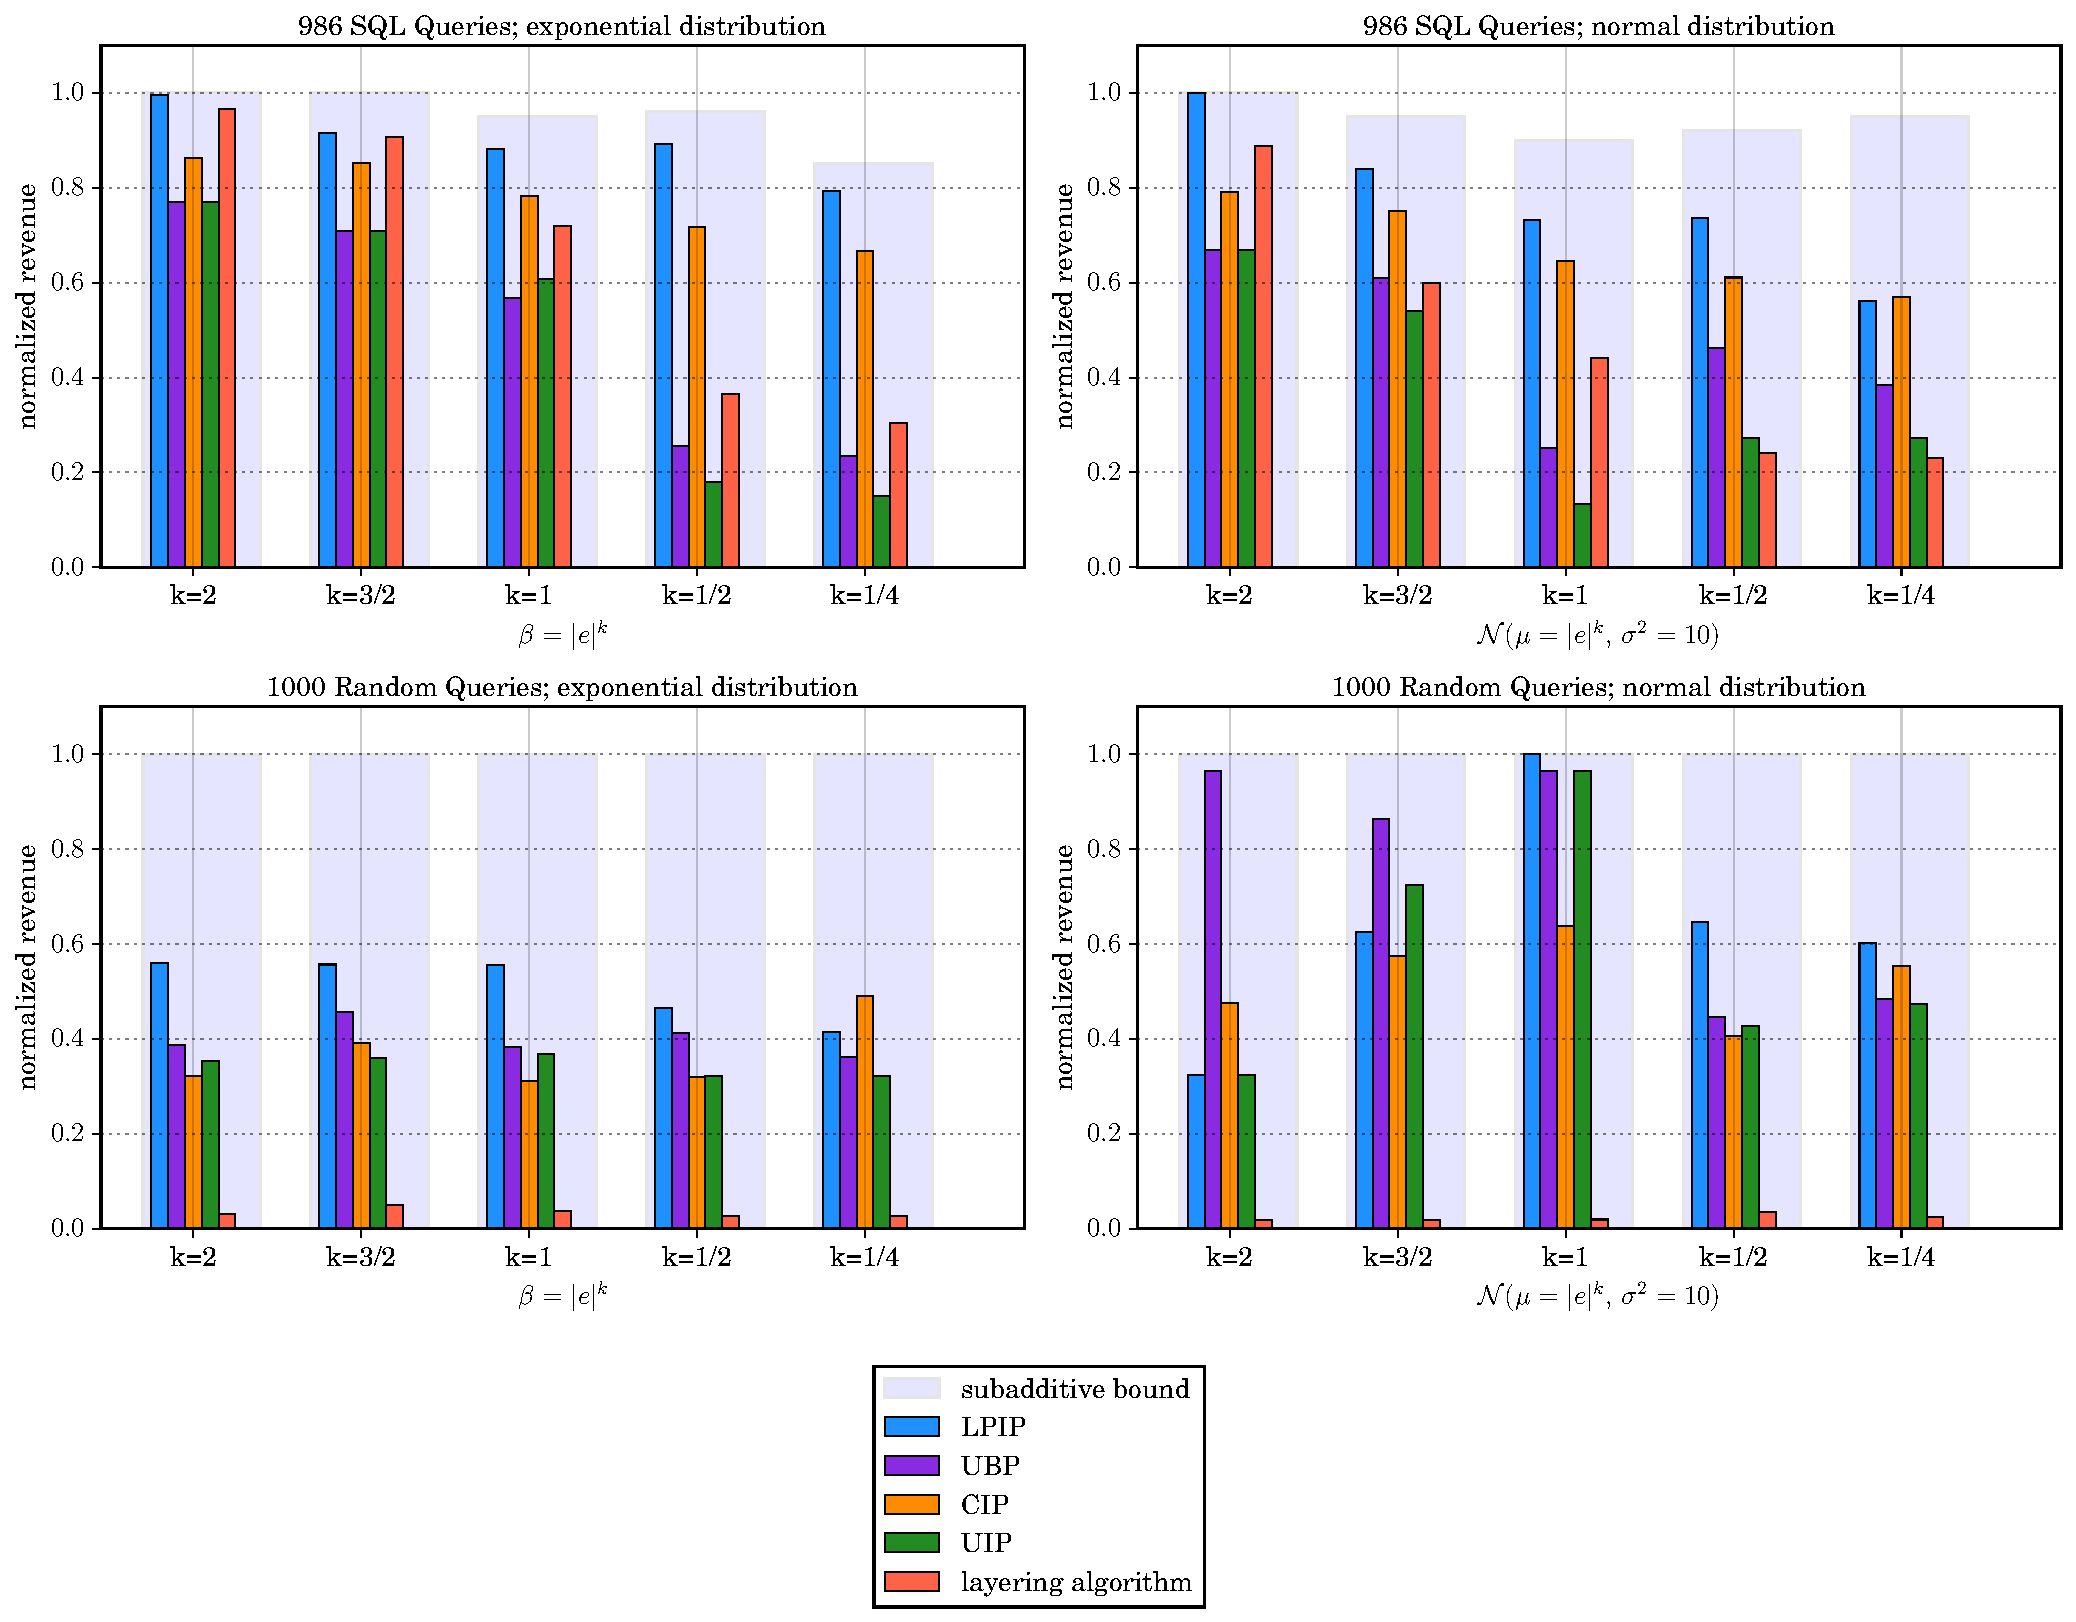
\includegraphics[scale=0.40]{queriesscalingedgesize.pdf}
	\caption{Scaling Bundle Valuations: SQL workload and random workload} \label{fig:scalingedge}
\end{figure}  

\subsubsection{Scaling Bundle Valuations} So far, the valuations are sampled independently of the edge size. Our next experiment will correlate the size of the edge with the valuation that is assigned to it. To this end, we will sample valuation from parameterized exponential and normal distribution as follows: we assign $v_e \sim {\rm exponential}(\beta = m^k)$ where $\beta$ is the mean of the distribution. Similarly, for normal distribution, $v_e \sim \mathcal{N}(\mu = m^k,\, \sigma^2 = 10)$. Here $k$ is the parameter that we will vary. Figure~\ref{fig:scalingedge} shows the result for different values of the parameter $k$. For both distributions, when $k \geq 1$, most of the revenue is concentrated in a few edges that have extremely large valuations. In this situation, $O(\log n + \log m)$-approximation algorithm and uniform bundle pricing perform well. We also investigate how XOS pricing functions behave. To define the function, we take the maximum over the best pricing vector generated by the item pricing algorithms. Not surprisingly, this does not give good results in our experiments. The last observation is to notice the approximation of uniform item pricing. The optimization of relaxing the uniform item prices via an LP dramatically increases the revenue extracted (sometimes by as much as 5x).

\subsubsection{Sampling Item Prices} The last of set of experiment on the SQL workload is to understand the behavior of algorithms when the valuation of edges is defined by an \emph{additive model}. More specifically, we define $k$ different distributions $\{D_i\}_{i=1}^{k}$ from which items will draw their prices and a special distribution $\tilde{D}$ which will assign each item which distribution it will sample from. The valuation of an edge is the defined as $v_e = \sum_{j \in e} x_j \sim D_{\ell_j}$ where $\ell_j \sim \tilde{D}$. Intuitively, this model will capture the scenario where parts of the database have non-uniform value and some parts are much more valuable than others. To see why this setting can be practical interest, consider a research analyst in banking who gives stock recommendations. While public information about companies and stocks may be cheap, the research analysts buy and sell recommendations will be of much higher value. For the purpose of experiments, we fix $D_i$ to $\textsf{Uniform}[i, i+1]$ and set $\tilde{D}$ to $\textsf{Uniform}[1, k]$ or $\textsf{Binomial}(k, 1/2)$ while varying $k$. Figure~\ref{fig:mixing} shows the results of this experiment. $O(\log m + \log n)$-approximation algorithm outperforms all other algorithms. For smaller values of $k$, the valuation of edges are close to additive (and exactly $m$ for $k=1$). In this case, there is no gap between uniform item pricing and its LP variant. As  the value of $k$ increases, uniform item pricing does slightly worse than the LP algorithm.


\begin{figure}[!t]
	\centering
	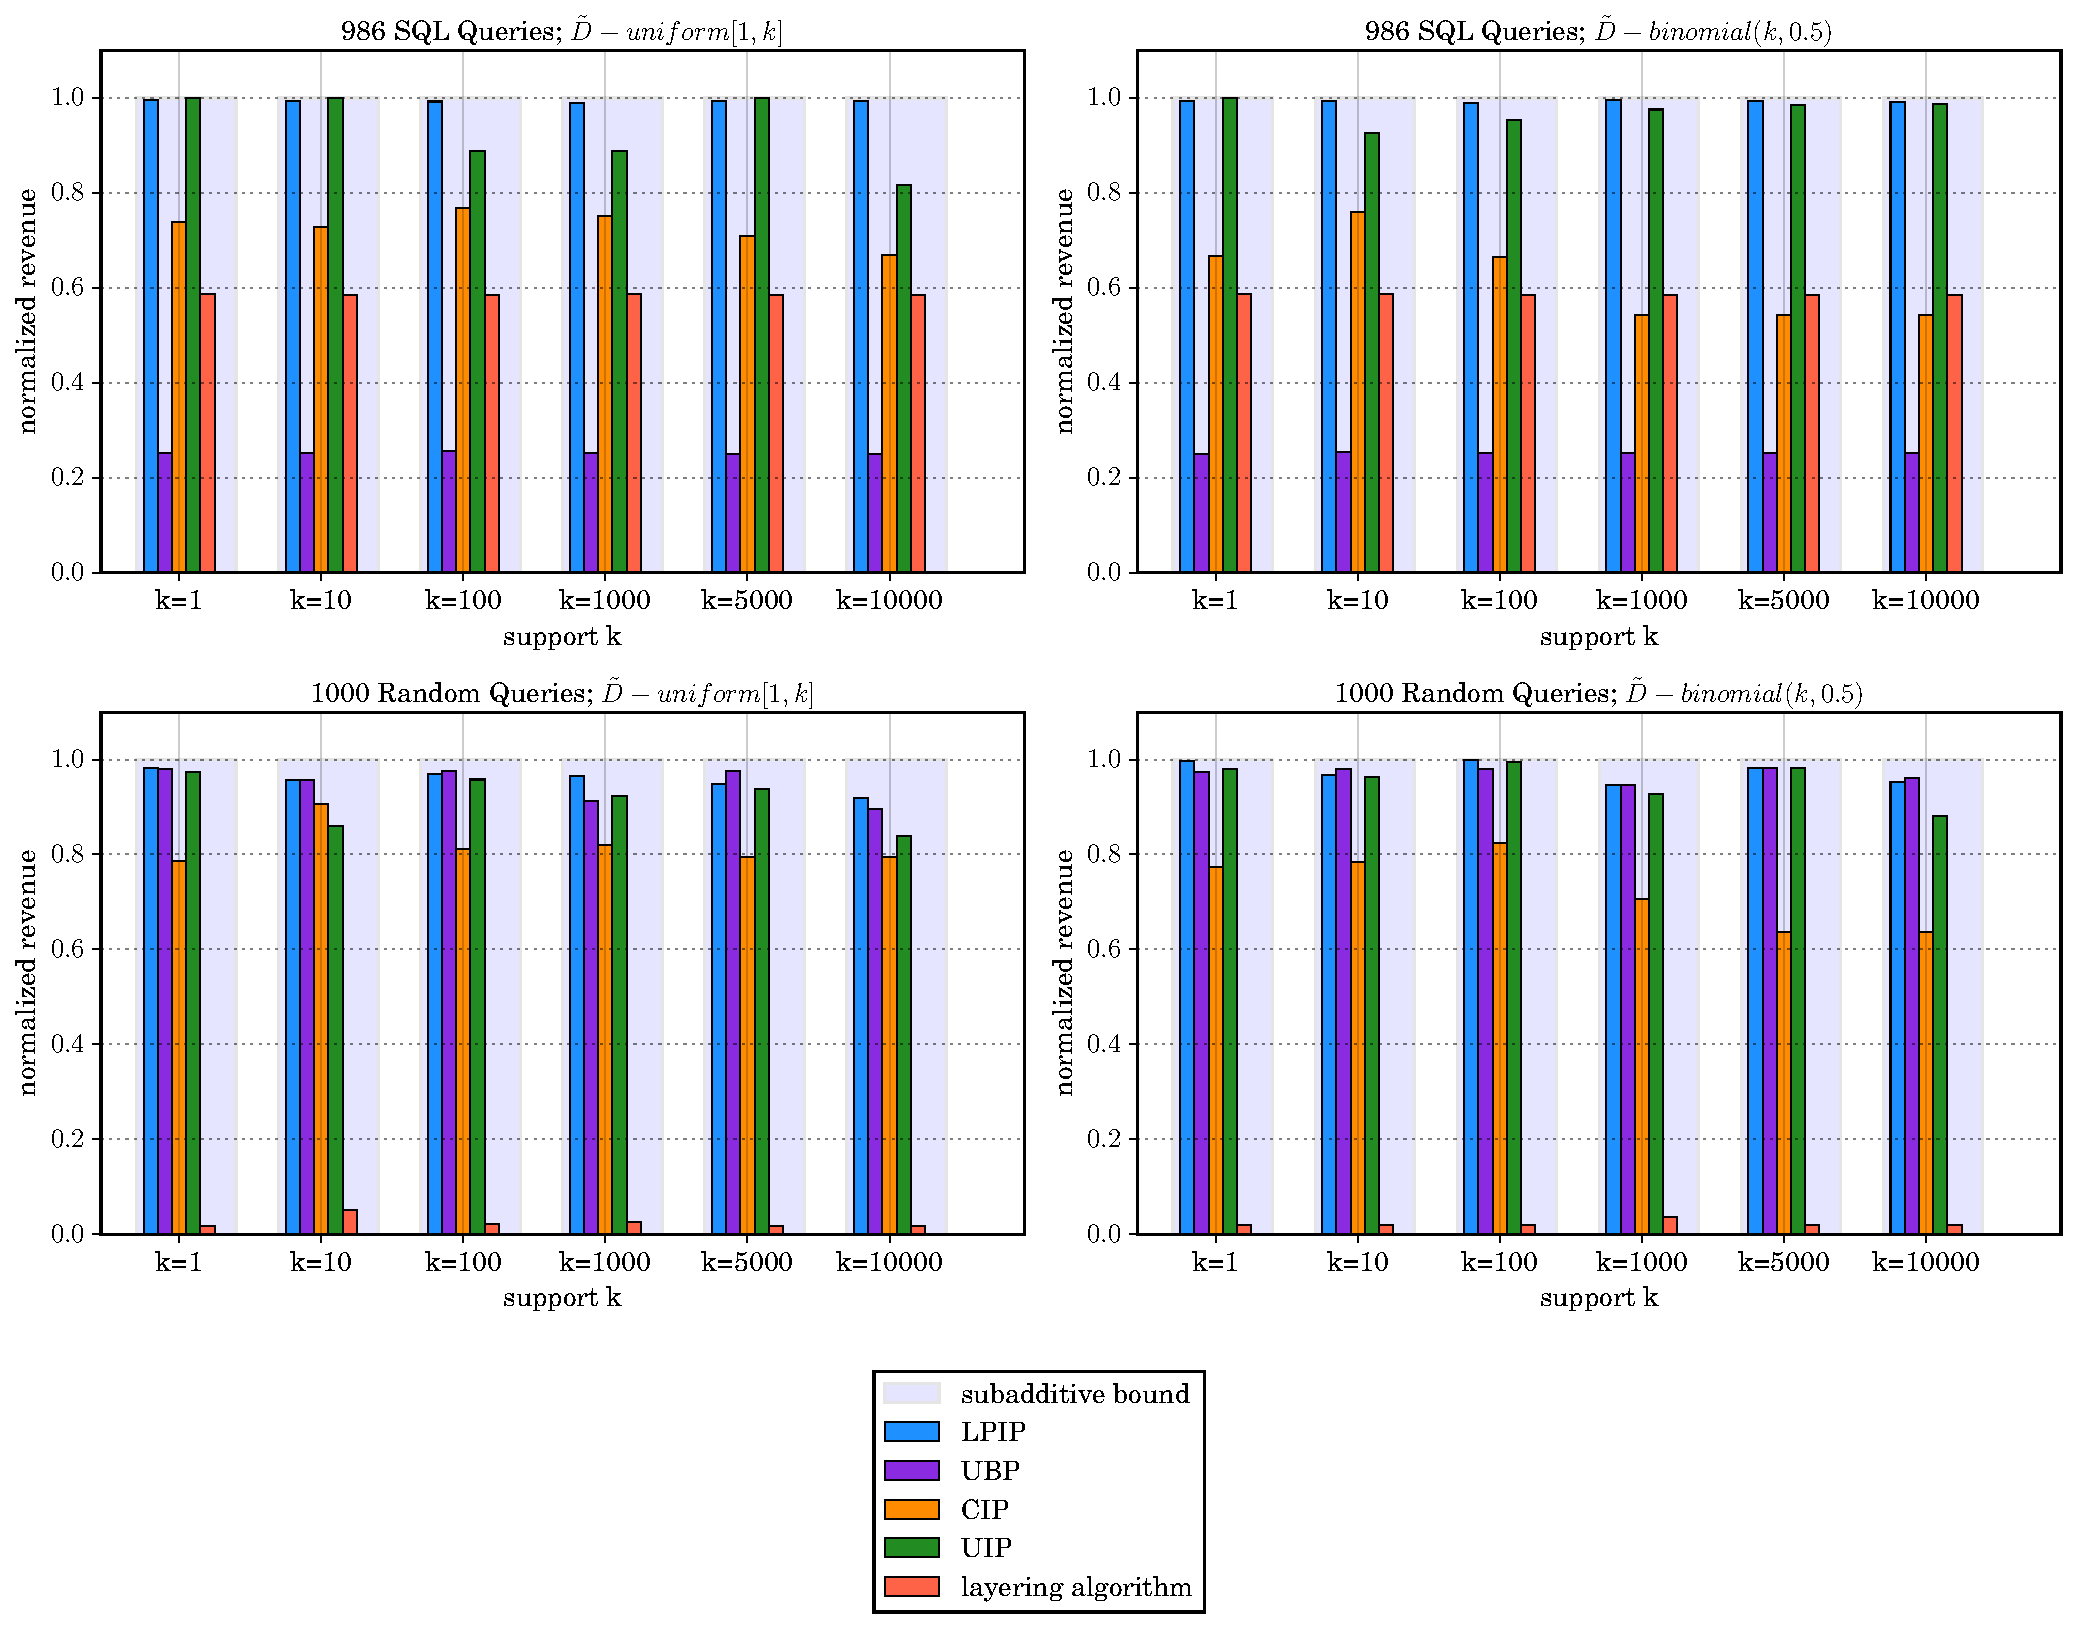
\includegraphics[scale=0.40]{queriesmixing.pdf}
	\caption{Sampling Item Prices: SQL workload and random workload} \label{fig:mixing}
\end{figure}  

\subsection{Experiment Results for Random Query Workload}


The second half of our experiments focuses on random query workload. For the following experiments, we generate $1000$ random queries and fix the resulting hypergraph. 

\subsubsection{Sampling Bundle Valuations}

In this experiment, valuations for each edge is chosen from the uniform distribution. Once again, uniform bundle pricing outperforms other approximation algorithms. Because of the high degree of overlap between hyperedges, the layering algorithm does not perform well as the number of levels formed is fairly large and thus, the algorithm cannot pack too many edges at any level.

\subsubsection{Scaling Bundle Valuations} In this valuation model, for random hypergraphs, uniform bundle pricing and $O(\log n+\log m)$-approximation algorithm are the best performing. The $O(\log B)$-approximation algorithm does not perform well even though it is theoretically optimal. This is because going over all capacity vectors with limited supply is extremely expensive. In our implementation, running the linear program for a large number of capacity vectors takes close to $2$ hours in total (we discuss reasons for this in the next section). Thus, we reduce the number of capacity vectors that we try by increasing the $(1+\epsilon)$ parameter. This introduces a factor of $(1+\epsilon)$ in the approximation ratio but allows for the running time to be smaller. Unfortunately, this factor is large enough to make the algorithm bad in practice. Note that we do not face this issue in the SQL workload since the largest degree item is shared by $22$ edges but random hypergraph has the largest degree close to $400$. The second row in Figure~\ref{fig:scalingedge} shows the results for random query workload. For the exponential distribution, no algorithm is close to optimal. We believe this is not an anomaly but rather the subaddtive bound not being as good as it should be.

\subsubsection{Sampling Item Prices} For this setting, all algorithms give a good approximation ratio except the layering algorithm. Bottom row in figure~\ref*{fig:mixing} shows the experimental results for random queries. Since the size of the edges is relatively concentrated, uniform item pricing and uniform bundle pricing do very well. Although $O(\log m + \log n)$ algorithm does the best, it does not improve by much since uniform item pricing gives a good baseline solution.  Once again, the layering algorithm is the worst performing out of all.


\subsection{Running Time of Algorithms}

\begin{table*}[] \centering
	%\ra{1.3}
	\begin{small}
		\begin{tabular}{@{}lrrrrr@{}}\toprule
			\textbf{Workload} & \textbf{LP} & \textbf{Uniform Bundle Pricing} & \textbf{Uniform Item Pricing} & $\mathbf{O(\log B)}$ & \textbf{Layering}  \\ \midrule
			
			\textbf{SQL Queries} &  60.62 & 15.50 & 25.45 & 812.67 & 15.67 \\ \hdashline
			\textbf{Random Queries} &  95.81 & 18.68 &  29.82 &1800 & 50.19 \\
			\bottomrule
		\end{tabular}
	\end{small}
	\caption{Algorithm running times (in seconds) for different workloads}
	\label{table:runtime}
\end{table*}

In this section we discuss the running time of the algorithms. Table~\ref{table:runtime} shows the run time of all algorithms for both the workloads. The most time efficient algorithms are uniform bundle pricing, uniform item pricing and the layering algorithm. Uniform bundle pricing and uniform item pricing depend only on number of hyperedges and the number of items in the hypergraph. Thus, they are very fast to run in practice. Layering algorithm is slightly slower but comparable in performance. Note that layering is faster on SQL workload as compared to the random hypergraphs since the maximum degree is much smaller. The two slowest running algorithms are $O(\log n + \log m)$-approximation and $O(\log B)$-approximation algorithm as they require running multiple linear programs. In practice, $O(\log n + \log m)$-approximation is faster than $O(\log B)$-approximation algorithm. This is because of the size of the linear program is very different. Observe that in our setting number of edges $m \sim 1000$ is much smaller than the number of items $n = 15000$. $O(\log n + \log m)$-approximation algorithm has $m$ constraints while $O(\log B)$-approximation algorithm has $n$ constraints. This dramatically influences the running time of the two algorithms. The $O(\log B)$-approximation algorithm uses $(1+\epsilon)$ as a parameter where $\epsilon$ controls the limited supply available for each item. We adjust the value of $\epsilon$ for both workloads to ensure that the running time is at most $30$ minutes. We fix $\epsilon = 0.2$ for SQL workload and $\epsilon = 4$ for random workload based on our empirical observations.
